\documentclass[french]{report}

% = = = = = = = = = =

\usepackage[T1]{fontenc}
\usepackage[utf8]{inputenc}

\usepackage{babel}

\usepackage{lscape}

% = = = = = = = = = =

\usepackage{titlesec}

\renewcommand\thechapter{\Roman{chapter}}

\titleformat\chapter
    {\normalfont\huge\bfseries}{\thechapter.}{1cm}{} 

\titleformat\section
    {\normalfont\Large\bfseries}{\thesection.}{.5cm}{}

% = = = = = = = = = =

% diagrammes de Gantt

\usepackage{pgfgantt}

% = = = = = = = = = =

% utilisation d'images

\usetikzlibrary{babel}

\graphicspath{{image/}}

% = = = = = = = = = =

% personnalisation des 'bullet point'
\usepackage{enumitem}

% = = = = = = = = = =

% utilisation des hyperliens
\usepackage{hyperref}

\hypersetup{
    colorlinks=true,
    linkcolor=blue,
    urlcolor=blue,
}

% = = = = = = = = = =

% utilisation du symbole euro
\usepackage{lmodern, textcomp}

% = = = = = = = = = =

\newcommand{\gamename}{\textbf{Fallen Dohyo} }

% = = = = = = = = = =

\title{\gamename\\Cahier des Charges Technique}
\author{Willy JACQUET \and Yoan PARRA }
\date{3 Mars 2019}

% = = = = = = = = = =

\begin{document}

\maketitle

\tableofcontents

\newpage

\chapter{Présentation}

    Ce projet s'inscrit dans le cadre de l'unité d'enseignement LIFAP4
    - Conception et développement d'applications,
    à l'université Claude Bernard Lyon 1, 
    sous la supervision d'Alexandre MEYER et de Nicolas PRONOST.

    L'objectif de ce projet est d'avoir un premier contact
    avec la conception et le développement d'applications,
    et ce, de manière formelle et rigoureuse.
    \linebreak
    Ce projet est mené par deux étudiants:
    \begin{itemize}
        \item Willy JACQUET, p1806811
        \item Yoan PARRA, p1505740
    \end{itemize}

    Relativement peu de restrictions sont imposées (cf. \ref{ch:contraintes}),
    nous avons choisi de concevoir et de développer un jeu vidéo.

    La suite de ce cahier décrit le jeu en question, les contraintes et le déroulement
    du projet, et enfin, en annexes, se trouve un diagramme de Gantt
    et un diagramme des classes.
    

\chapter{Description, \textit{Ten-Pager}}

\section{Présentation}

    \gamename est jeu vidéo de combat et de platforme multijoueur
    mettant en scène deux joueurs dans une arène dont le but est d'éjecter
    l'autre.
    \linebreak
    Jeux similaires:
    \begin{itemize}[label=$\bullet$]
        \item Céleste
        \item Super Meat Boy
        \item Super Smash Bros
        \item Tower Fall
    \end{itemize}

\section{Personnage}

    Vous incarnez un esclave moderne de la société;
    harcelé et exploité par votre patron, le mariage en péril...

\begin{center}
    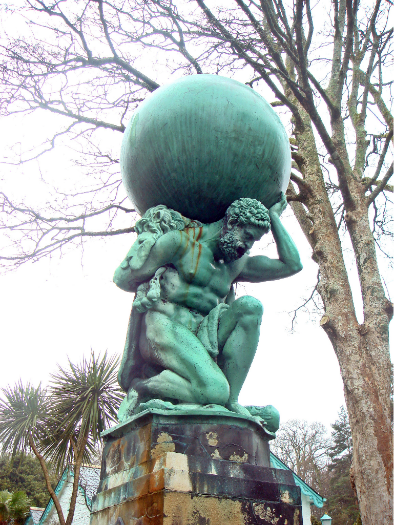
\includegraphics[width=5cm]{hercules}
\end{center}

    Au détour d'un coin perdu,
    vous entendez des hurlements de rage.
    Vous découvrez ainsi une arène sauvage,
    où tous sont aussi pathétiques que vous.
    Vous enlevez votre costume, le pliez et le posez.
    Vous joignez ces affrontements dénués de sens;
    vous allez vous lavez de l'humiliation
    qui vous a été faite.

\section{Jouabilité}

    \gamename se joue avec peu de contrôles.
    Deux joueurs peuvent jouer sur un même clavier.

    Les contrôles consitent en quatre commandes directionnelles
    et une commande pour foncer, ainsi qu'un bouton pause.

\section{Univers}

    Les arènes de \gamename se situent
    à différents endroits du monde,
    à l'abri des regards;
    là, où des hommes n'ont aucune valeur.

\begin{center}
    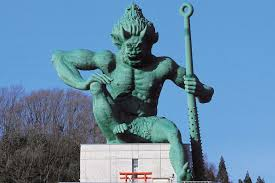
\includegraphics[width=8cm]{oni}
\end{center}

\section{Expérience, \textit{Gestalt}}

    En quelques secondes, deux joueurs peuvent débuter une partie.
    Les contrôles se veulent réactifs et nerveux.

    \gamename est un défouloir excitant et compétitif
    épousant la loi de Bushnell: \textit{easy to learn, hard to master}.

\section{Mécaniques}

\begin{center}
    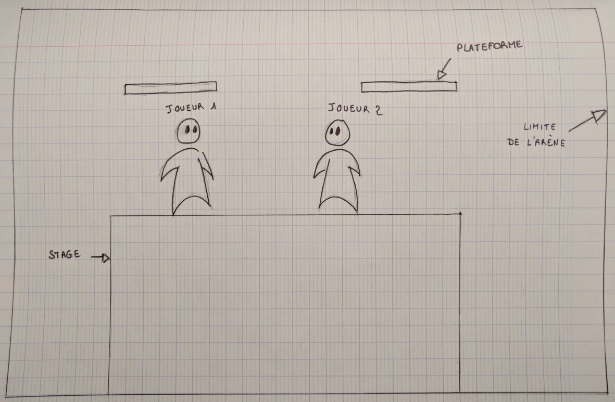
\includegraphics[width=12cm]{stage}
\end{center}

\begin{itemize}[label=$\bullet$]
    \item \textbf{Charge.}
    
    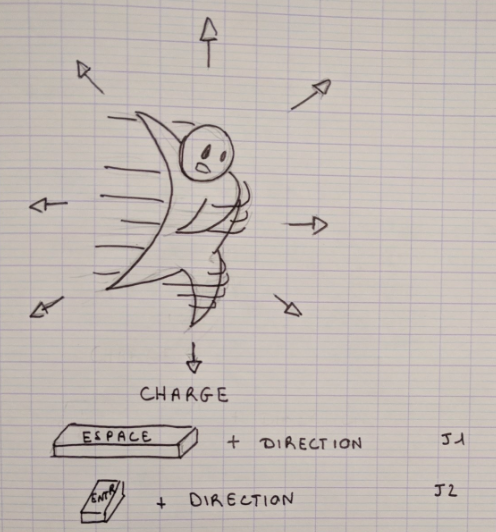
\includegraphics[width=8cm]{dash}

    \newpage
    \item \textbf{Déplacements.}
    
    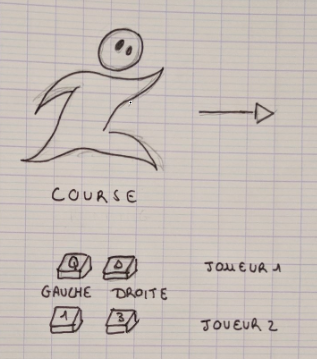
\includegraphics[width=5cm]{run}
    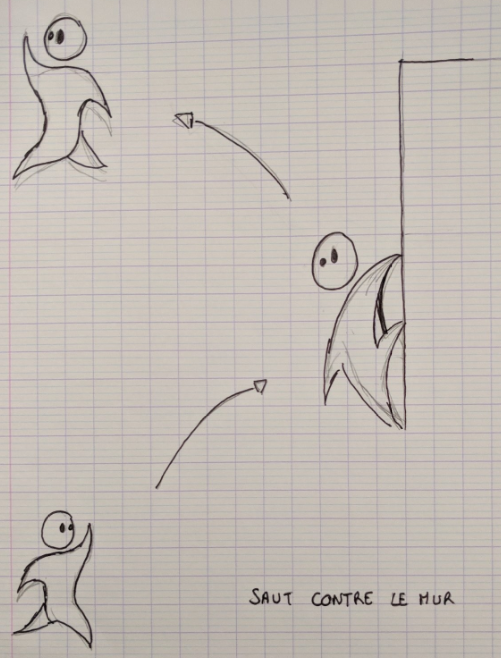
\includegraphics[width=5cm]{wall_jump}

    \item \textbf{Éjection.}
    
    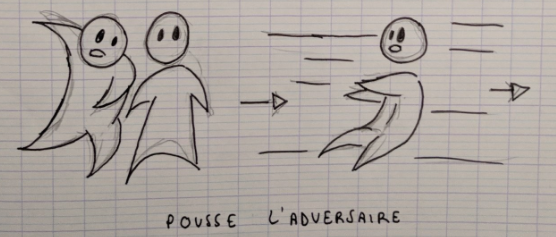
\includegraphics[width=10cm]{push}

    \newpage
    \item \textbf{Saut.}
    
    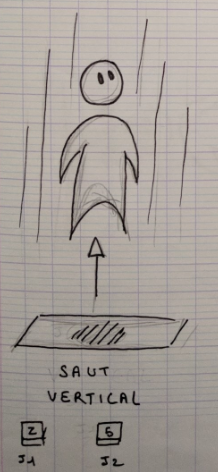
\includegraphics[width=4cm]{jump}
    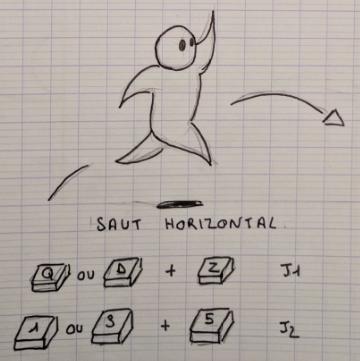
\includegraphics[width=6cm]{leap}

\end{itemize}

\section{Rejouabilité}

    \gamename est un jeu d'arcade multijoueur,
    les parties sont rapides et sans prérequis,
    il sera donc joué occasionnellement entre amis,
    tel un jeu d'arcade, ou en compétition.

\section{Modèle économique}

    L'objectif financier de \gamename n'est pas de générer un bénéfice
    mais de rembourser les coûts de développement
    et de gagner en visibilité dans le secteur du jeu vidéo.
    Le produit sera vendu de manière unitaire pour une durée illimitée.

    Le produit ne comportera pas de microtransations ou d'extensions payantes
    car nous, les développeurs, sommes hostiles à ces pratiques
    et mettons un point d'honneur à ne pas les implémenter.
    Des mises à jour corretives seront distribuées gratuitement.
    Le prix estimé du produit devrait être dans la tranche de 2€ à 5€.
    
    Seules des copies dématérialisées seront distribuées,
    c'est à dire qu'il n'y aura pas de production d'un support physique du produit.
    La distribution du produit sera confiée à une plarforme tiers,
    telle que Steam ou GOG.

\chapter{Contraintes}\label{ch:contraintes}

    Le produit final, ainsi que sa conception et sa réalisation,
    est soumis à des consignes dont le détail est disponible
    au terme les liens suivants:
    \begin{itemize}[label=$\bullet$]
        \item \href{https://docs.google.com/spreadsheets/d/1OcpRm6gQtmRNWSXeG7QwnFJ6Eqzl7_DKCjUM4V9P4A0/edit#gid=1}
        {Barême de notation}
        \item \href{https://perso.liris.cnrs.fr/alexandre.meyer/public_html/www/doku.php?id=lifap4}
        {LIFAP4 - Conception et développement d'applications}
    \end{itemize}

\section{Livrables}

    Le produit final est constitué
    d'un exécutable pour les systèmes Windows (.exe)
    et de bibliothèques de liens dynamiques (.dll),
    d'un éxécutable pour les systèmes GNU Linux (.out),
    des sources
    ainsi que de la documentation technique et fonctionnelle.

\section{Temporalité}

    La réalisation du produit s'effectuera du mardi 26 février 2019 au mardi 6 mai 2019.
    \begin{itemize}[label=$\bullet$]
        \item jeudi 7 mars 2019, dépôt du cahier des charges technique
        sur la platforme Tomuss.
        \item mardi 26 mars 2019, présentation de la démonstration intermédiaire.
        \item lundi 6 mai 2019, dépôt du produit final sur la platforme Tomuss.
        \item mardi 7 mai 2019, présentation du produit final.
    \end{itemize}

\section{Budget}

    Aucune rémunération, ni aide monétaire n'est prévu
    pendant ou à terme de la réalisation du produit.
    Par conséquent en tant qu'étudiants, nous, les développeurs, 
    ne pourrons pas accorder plus de quelques dizaines d'euros à la réalisation du produit.

    Ce budget sera investit principalement dans l'achat de ressources graphiques
    (scènes, textures, \textit{sprites sheet}, etc)
    et audio (effets sonores, musiques, etc).

\chapter{Déroulement}

\section{Implémentation}

    Le language de programmation utilisé est le C++.

    Le code source et la documentation technique sont en anglais,
    tandis que la documentation fonctionnelle est en français.
    
    Les bilbiothèques \textit{Standard Template Library}
    et \textit{Simple and Fast Multimedia Library}
    sont utilisés à divers usages.

\section{Tâches}

\begin{enumerate}
    \item \textbf{Écriture du makefile.}
    
    Fichier ./makefile.

    Cibles pour les éxécutables, la documentation et le nettoyage.
    
    \item \textbf{Écriture du readme.}
    
    Fichier ./readme.md.

    Introduction au projet;
    à son usage, à ses dépendances, à sa politique, à sa documentation.

    \item \textbf{Création du Doxyfile.}
    
    Fichier ./doc/Doxyfile.

    Configuration de la génération automatique de la documentation.

    \item \textbf{Écriture du cahier des charges.}
    
    Fichiers ./doc/technical\_specification/*.

    Cahier des charges techniques,
    diagramme de Gantt, diagramme des classes.

    \item \textbf{Conception du module Audio.}
    
    Fichiers ./src/audio/*.

    Gestion, stockage et chargement
    des sons, des musiques et des effets sonores.

    Liaison avec la bibliothèque SFML.

    \item \textbf{Conception du module Graphics.}
    
    Fichiers ./src/graphics/*.

    Gestion, stockage et chargement
    des fenêtres, des sprites, des textures,
    des caméras et des shaders.

    Affichage de la fenêtre et des éléments graphiques.

    Liaison avec la bibliothèque SFML.

    \item \textbf{Conception du module Logic.}
    
    Fichiers ./src/prototype/*, ./src/logic/*.

    Gestion du déroulement du jeu.
    Logique interne, implémentation du gamplay.

    Création nombreuses de prototypes.

    Dépend du module Physics.

    \item \textbf{Conception du module Physics.}
    
    Fichiers ./src/physics/*.

    Outils pour la résolution
    de problèmes mathématiques ou physiques.

    Détection et réponses des collisions,
    mécanique classique (position, vitesse, accélération).
    
    \item \textbf{Conception du module System.}
    
    Fichiers ./src/system/*.

    Coordination des différents modules entre eux.

    Élément central de l'application.
    
    \item \textbf{Conception du module UI.}
    
    Fichiers ./src/UI/*.

    Éléments intéractifs (boutons, menus, texte),
    gestion de la souris, du clvaiers et des joysticks.

    Dépend du module Graphics.
    
    \item \textbf{Conception de la démonstration intermédiaire.}
    
    Fichier ./bin/demonstration.(exe/out).

    Éxécutable qui sera présenté lors de la démonstration.
    
    \item \textbf{Conception du produit final.}
    
    Fichier ./bin/final.(exe/out).

    Éxécutable contenant le jeu final.

    Nettoyage des sources.


\end{enumerate}

\chapter{Annexes}

\begin{landscape}
\section{Diagramme de Gantt}
\begin{ganttchart}[
    vgrid={*3{dotted}}, x unit = 0.5cm, y unit chart = .7cm
]{1}{33}
    \gantttitle{25/02}{3}
    \gantttitle{04/03}{3}
    \gantttitle{11/03}{3}
    \gantttitle{18/03}{3}
    \gantttitle{25/03}{3}
    \gantttitle{01/04}{3}
    \gantttitle{08/04}{3}
    \gantttitle{15/04}{3}
    \gantttitle{22/04}{3}
    \gantttitle{29/04}{3}
    \gantttitle{06/04}{3} \\
    \ganttbar{makefile}{1}{3} \\
    \ganttbar{Cahier des charges}{1}{5} \\
    \ganttbar{readme}{3}{5} \\
    \ganttbar{Module Physics}{3}{12} \\
    \ganttbar{Doxyfile}{4}{5} \\
    \ganttbar{Module Logic}{6}{15} \\
    \ganttbar{Module Graphics}{9}{24} \\
    \ganttbar{Module System}{11}{25} \\
    \ganttbar{Démonstration}{13}{16} \\
    \ganttbar{Module UI}{15}{27} \\
    \ganttbar{Module Audio}{21}{28} \\
    \ganttbar{Produit final}{24}{31} \\
\end{ganttchart}
\end{landscape}

\section{Diagramme des classes}
\makebox[\textwidth][c]{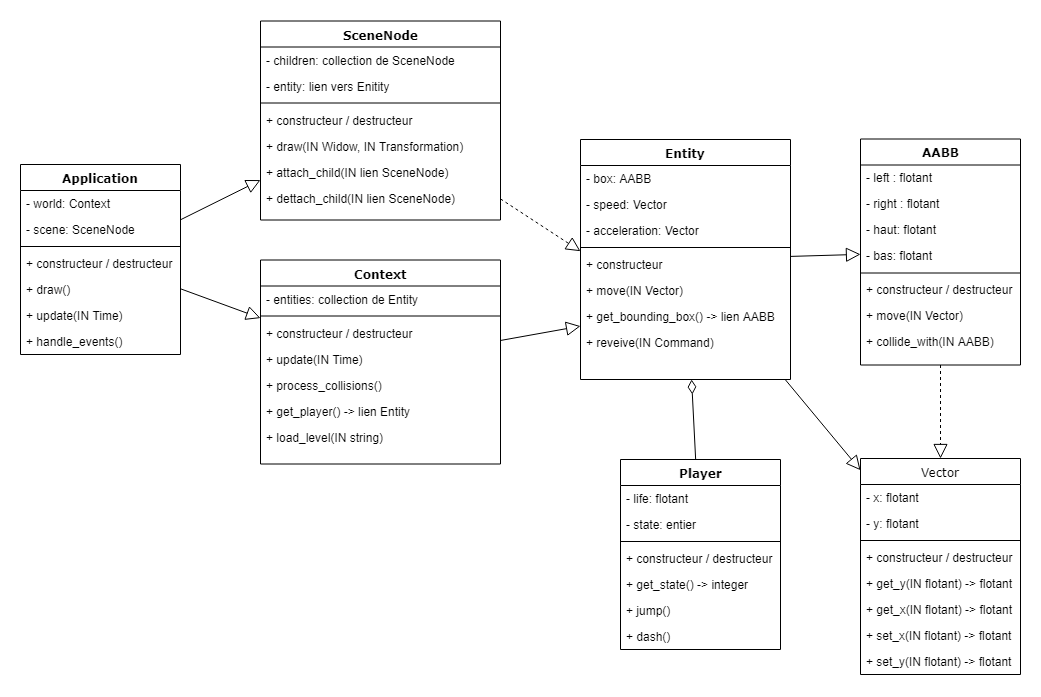
\includegraphics[width=20cm]{uml}}

\end{document}
 